\documentclass{article}
\usepackage[utf8]{inputenc}
\usepackage{amsmath}
\usepackage{graphicx}
\usepackage[spanish]{babel}                                 % Spanish dictionary.
\usepackage[utf8]{inputenc}                                 % Ñ's in text.
\usepackage{tabu}
\usepackage{graphicx}
\usepackage{caption}
\usepackage{subcaption}
\usepackage{amsmath}
\usepackage{listings}
\title{Tarea 02: Determinación de la complejidad de los problemas}
\author{Álvaro Antonio Soto Escobar\\Jorge Carlos Urteaga Reyesvera }
\date{August 2016}

\begin{document}

\maketitle

\section{Demostraciones}
Demostrar si las siguientes funciones son $\Theta(N^2)$ y encontrar los valores de $c_1$, $c_2$, $n$ y $n_0$ para cada una de las funciones. Para eso es necesario definir una función de orden 2 vista en clase.

\begin{gather*} 
 f(n)=an^2+bn+c\\ 
 c_1 \leq an^2+bn+c\leq c_2 \quad \quad\forall n>n_0\\
 c_1 = \cfrac{a}{4}\\
 c_2= \cfrac{7a}{4}\\
 n_0 = 2\cdot\max{\cfrac{|b|}{a}\geq \sqrt{|c|/a }}
\end{gather*}

\begin{enumerate}
    \item $60n^2 + 5n + 1 $
\begin{gather*} 
 f(n)=60n^2 + 5n + 1 \\ 
 c_1 \leq 60n^2 + 5n + 1 \leq c_2 \quad \quad\forall n>n_0\\
 c_1 = \cfrac{60}{4}=15\\
 c_2= \cfrac{7\cdot 60}{4}=105\\\\
 n_0 = 2\cdot\max{\cfrac{|5|}{60}\geq \sqrt{|1|/60 }}\\
 = 2\cdot\max{0.083333, 0.129099}
 = 2\cdot0.129099 = 0.25
 \end{gather*}

Para que se cumpla la condición $n=1$, por lo que queda de la siguiente manera:

\begin{gather*} 
 15 \leq 60n^2 + 5n + 1 \leq 105 \\
 \forall n \geq 1
 \end{gather*}

    \item $2x^2-16x +35$
\begin{gather*} 
 f(n)=2x^2-16x +35 \\ 
 c_1 \leq 2x^2-16x +35 \leq c_2 \quad \quad  \forall n>n_0\\
 c_1 = \cfrac{2}{4} = \cfrac{1}{2}\\
 c_2= \cfrac{7\cdot 2}{4}=\cfrac{7}{2}\\
 n_0 = 2\cdot\max{\cfrac{|16|}{2}\geq \sqrt{|35|/1 }}\\
 = 2\cdot\max{8, 4.183300}
 = 2\cdot 8 = 16
\end{gather*}
Para que se cumpla la condición $n=1$, por lo que queda de la siguiente manera:

\begin{gather*} 
 \cfrac{1}{2} \leq 2x^2-16x +35 \leq \cfrac{7}{2} \\
 \forall n \geq 1
 \end{gather*}


    \item $3n^2 + 2n \cdot \log_2 n$
    
\begin{gather*} 
 f(n)=3n^2 + 2n \cdot \log_2 n\\ 
 c_1 \leq 3n^2 + 2n \cdot \log_2 n \leq c_2\quad \quad\forall n>n_0\\
 c_1 \leq 3 + 2 \cfrac{\log_2 n }{n} \leq c_2 \\
 \text{Tip: Debido a que suponemos que $c=k$,ajustamos para que $c_1=3$, pues la constante es 3.} \\
 \text{En el caso de C2, si sabemos que la funcińn logaritmica tienda a 1.1, podemos actoar $c_2=5$ } \\
 \text{ Por las limitaciones de la función logaritmica sabemso que n tiene que ser mayor a uno} \\
 c_1 = 3\\
 c_2= 5\\
 n_0 = 1
\end{gather*}

    \item $2 + 4 + 6 \dots 2n$ Esta función se puede ver como la siguiente sumatoria
    
\begin{gather*} 
 2 +  4 +6 + \dots + 2n\\
 = 2 ( 1 + 2 + 3 + \dots n)\\
 = 2 \sum_{i=1}^{n}i = 2\cfrac{n(n+1)}{2}\\
 = n(n+1) = n^2 + n \\
 \end{gather*}
 \begin{gather*} 
 f(n)=n^2 + n  \\ 
 c_1 \leq n^2 + n  \leq c_2 \quad \quad  \forall n>n_0\\
 c_1 = \cfrac{1}{4} = 0.25\\
 c_2= \cfrac{7\cdot 1}{4}=\cfrac{7}{4}\\
 n_0 = 2\cdot\max{\cfrac{|1|}{1}\geq \sqrt{|0|/1 }}\\
 = 2\cdot\max{1, 0}
 = 2\cdot 1 = 2
\end{gather*}

Finalmente:

\begin{gather*} 
    \cfrac{1}{4} \leq n^2 + n \leq \cfrac{7}{4}
    \cfrac{1}{4} \leq 1 + \cfrac{1}{4} \leq \cfrac{7}{4}
 \forall n \geq 1
 \end{gather*}
    \item la siguiente expresión:
\begin{lstlisting}[language=Python]
for i = 1 to n  
    for j = 1 to i
        for k=1 to s
            x = x+1
\end{lstlisting}
De acuerdo a la clase, el ciclo d ejecución del \textit{for} se ejecuta $n+1$. Para este ejercicio suponemos dos escenarios. el primero donde el tamaño del cilo es n, es decir iguales y el segundo donde el tamaño del ciclo es aumenta, 
\begin{lstlisting}[language=Python]
A )for i = 1 to n       Costo c_1 es n +1  veces
    B ) for j = 1 to i  Costo c_2 es i+1 veces por cada ciclo de A
        C) for k=1 to j Costo c_3 es k+1 veces por cada ciclo de B
          D)   x = x+1  Costo c_4 1 veces por cada ciclo de C
\end{lstlisting}
\begin{itemize}
\item  Tamaño

En el caso de un sólo ciclo for  se sabe que su complejidad es $n+1$, esto se puede ver como
\begin{equation*}
    \sum_{i=1}^{n+1} 1 = n+1
\end{equation*}
En el caso de dos for anidados de tamaño $n$
\begin{equation*}
    \sum_{i=1}^{n+1}\sum_{j=1}^{n+1} 1 = \sum_i^{n+1}= (n+1) = (n+1)^2
\end{equation*}
Para tres, el del ejercicio

\begin{equation*}
    \sum_{i=1}^{n+1}\sum_{j=1}^{n+1}\sum_{k=1}^{n+1} 1 = (n+1)^3
\end{equation*}
Para $n$
\begin{equation*}
    \sum_{i=1}^{n+1}\sum_{j=1}^{n+1}\dots \sum_{z=1}^{n+1} 1 = (n+1)^n
\end{equation*}
\item Tamaño variable

En el caso de dos for anidados.
\begin{equation*}
    \sum_{i=1}^{n+1}\sum_{j=1}^{i+1} 1 = \sum_{i=1}^{n+1} i= 1 + 2 +\dots n = \cfrac{n(n+1)}{2}
\end{equation*}
En el caso de tres for anidados.
\begin{equation*}
    \sum_{i=1}^{n+1}\sum_{j=1}^{i+1}\sum_{k=1}^{j+1} 1 = \sum_{i=1}^{n+1}\sum_{j=1}^{i+1} j= \cfrac{n(n+1)}{2}
\end{equation*}
\begin{equation*}
     \sum_{i=1}^{n+1}\sum_{j=1}^{i+1} i= \sum_{i=1} i^2 = \cfrac{n(n+1)(2n+1)}{6}
\end{equation*}

En el caso de cuatro for anidados.
\begin{equation*}
    \sum_{i=1}^{n+1}\sum_{j=1}^{i+1}\sum_{k=1}^{j+1}\sum_{l=1}^{k+1} 1  = (\sum_{i=1}^2 x)^2
\end{equation*}
A esta sucesión se llama fórmula de Faulhaber que se pueden describir con los polinomios de Bernoulli. La siguiente imagen la complejidad de los problemas se extiende a polinomios de grado 3.
\end{itemize}
\end{enumerate}
%% Versión Alvaro

\section{Gráficas}
Dado un conjunto de funciones ordenarlas de acuerdo a la tasa de crecimiento

\begin{enumerate}
    \def\labelenumi{\arabic{enumi}.}
    \itemsep1pt\parskip0pt\parsep0pt
    \item $\textrm{lg}(\textrm{lg}^*(n))$
    \item $2^{\textrm{lg}^*(n)}$
    \item $\sqrt{2}^{\textrm{lg}(n)}$
    \item $n^2$
    \item $n!$
    \item $(\textrm{lg}(n))!$
    \item $(\frac{3}{2})^n$
    \item $n^3$
    \item $\textrm{lg}^2(n)$
    \item $\textrm{lg}(n!)$
    \item $2^{2^{n}}$
    \item $n^{\frac{1}{\textrm{lg}(n)}}$
    \item $\ln(\ln(n))$
    \item $\textrm{lg}^*(n)$
    \item $n 2^n$
    \item $n^{\textrm{lg}( \textrm{lg}(n))}$
    \item $\ln (n)$
    \item $1$
    \item $2^{\textrm{lg}(n)}$
    \item $\textrm{lg}(n)^{\textrm{lg}(n)}$ 
    \item $e^n$
    \item $4^{\textrm{lg}(n)}$ 
    \item $(n+1)!$
    \item $\sqrt{\textrm{lg}(n)}$
    \item $\textrm{lg}^*(\textrm{lg}(n))$
    \item $2^{\sqrt{2 \textrm{lg}(n)}}$
    \item $n$
    \item $2^n$
    \item $n\textrm{lg}(n)$ 
    \item $2^{2^{n+1}}$
\end{enumerate}

\begin{enumerate}
\item Primero podemos intentar resolver este ejercicio generando un código y llevando las funciones al punto de quiebre en el limite en \infty.

\begin{lstlisting}[language=Python]
graphs.append(('grafica30', '2^2^(n+1)', 2**(2**(val+1)) ))
graphs.append(('grafica11', '2^(2^n)', 2**(2**val) ))
graphs.append(('grafica23', '(n+1)!', factorial(val+1) ))
graphs.append(('grafica5', 'n!', factorial(val) ))
graphs.append(('grafica21', 'exp(n)', np.exp(val) ))
graphs.append(('grafica15', 'n*2^n', val*(2**val) ))
graphs.append(('grafica28', '2^n', 2**val ))
graphs.append(('grafica7', '(3/2)^n', (3.0/2.0)**val ))
graphs.append(('grafica20', '(Log(n))^(Log(n))', (np.log2(val))**(np.log2(val)) ))
graphs.append(('grafica16', 'n^(log(log n))', val**(np.log2(np.log2(val))) ))
graphs.append(('grafica6', '(Log(n))!', factorial(np.log2(val)) ))
graphs.append(('grafica8', 'n^3', val**3 ))
graphs.append(('grafica4', 'n^2', val**2 ))
graphs.append(('grafica22', '4^(Log(n))', 4**np.log2(val) ))
graphs.append(('grafica10', 'Log(n!)', np.log2(factorial(val)) ))
\end{lstlisting}

\item Después eliminamos las gráficas ya ordenadas de la lista y con variaciones de los valores de 'X' (agregando 0s) hasta 10000000000000000000 se logro este orden

\begin{lstlisting}[language=Python]
graphs.append(('grafica29', 'n*(Log(n))', val*np.log2(val) ))
graphs.append(('grafica19', '2^(Log(n))', 2**np.log2(val) ))
graphs.append(('grafica27', 'n', val ))
graphs.append(('grafica3', 'sqrt(2)^Log(n)', np.sqrt(2)**np.log2(val) ))
\end{lstlisting}

\item Con las gráficas que quedaron notamos que con valores extremadamente grandes, crecen lento, pero con diferencia considerable como para considerar el orden.

\begin{lstlisting}[language=Python]
graphs.append(('grafica26', '2^sqrt(2*Log(n))', 2**(np.sqrt(2*np.log2(val))) ))
graphs.append(('grafica9', 'Log^2(n)', (np.log2(val))**2 ))
\end{lstlisting}

\item Después se ve que las gráficas crecen extremadamente lento y con diferencia despreciable entre ellas, por lo que no existe posibilidad de que cambien de orden

\begin{lstlisting}[language=Python]
graphs.append(('grafica17', 'Ln(n)', np.log(val) ))
graphs.append(('grafica24', 'sqrt(Log(n))', np.sqrt(np.log(val)) ))
graphs.append(('grafica13', 'Ln(Ln(n))', np.log(np.log(val)) ))
\end{lstlisting}

\item Con las gráficas de logaritmo iterado, notamos que: se vuelven estables cuando x tiende a infinito ya que log*(x) vale máximo 5 y es de lento crecimiento, de acuerdo a la siguiente tabla:

\begin{table}[h]
    \centering
    \label{my-label}
    \begin{tabular}{|l|l|}
    \hline
        x                                  & lg*(n) \\ \hline
        (-\infty, 1{]}                          & 0       \\ \hline
        (1, 2{]}                           & 1       \\ \hline
        (2, 4{]}                           & 2       \\ \hline
        (4, 16{]}                          & 3       \\ \hline
        (16, 65536{]}                      & 4       \\ \hline
        (65536, 2\textasciicircum 65536{]} & 5       \\ \hline
    \end{tabular}
    \caption{Valores de lg*(n)}
\end{table}

\begin{lstlisting}[language=Python]
graphs.append(('grafica2', '2^(Log*(n))', 2.0**logstar(val) ))
graphs.append(('grafica14', 'Log*(n)', logstar(val) ))
graphs.append(('grafica25', 'Log*(Log(n))', logstar(np.log2(val)) ))
graphs.append(('grafica1', 'Log(Log*(n))', np.log2(logstar(val)) ))
\end{lstlisting}

\item Las últimas, se ordenan por si solas por su bajo o nulo crecimiento

\begin{lstlisting}[language=Python]
graphs.append(('grafica12', 'n^(1/Log(n))', val**(1.0/np.log2(val)) ))
graphs.append(('grafica18', '1', 1 ))
\end{lstlisting}

\end{enumerate}

El orden final de las funciones es el siguiente.

\begin{enumerate}
    \def\labelenumi{\arabic{enumi}.}
    \itemsep1pt\parskip0pt\parsep0pt
    \item $2^{2^{n+1}}$
    \item $2^{2^{n}}$
    \item $(n+1)!$
    \item $n!$
    \item $e^n$
    \item $n 2^n$
    \item $2^n$
    \item $(\frac{3}{2})^n$
    \item $\textrm{lg}(n)^{\textrm{lg}(n)}$ 
    \item $n^{\textrm{lg}( \textrm{lg}(n))}$
    \item $(\textrm{lg}(n))!$
    \item $n^3$
    \item $n^2$
    \item $4^{\textrm{lg}(n)}$ 
    \item $\textrm{lg}(n!)$
    \item $n\textrm{lg}(n)$ 
    \item $2^{\textrm{lg}(n)}$
    \item $n$
    \item $\sqrt{2}^{\textrm{lg}(n)}$
    \item $2^{\sqrt{2 \textrm{lg}(n)}}$
    \item $\textrm{lg}^2(n)$
    \item $\ln (n)$
    \item $\sqrt{\textrm{lg}(n)}$
    \item $\ln(\ln(n))$
    \item $2^{\textrm{lg}^*(n)}$
    \item $\textrm{lg}^*(n)$
    \item $\textrm{lg}^*(\textrm{lg}(n))$
    \item $\textrm{lg}(\textrm{lg}^*(n))$
    \item $n^{\frac{1}{\textrm{lg}(n)}}$
    \item $1$
\end{enumerate}

\clearpage
Gráficamente las funciones se visualizan de la siguiente manera.

\fbox{
  \parbox{\textwidth}{
Tomar en cuenta que las gráficas toman el orden expuesto cuando x tiende a infinito, esto es solo un ejemplo de como se comportan las funciones.
  }
}

\begin{figure}[h]
 
\begin{subfigure}{0.5\textwidth}
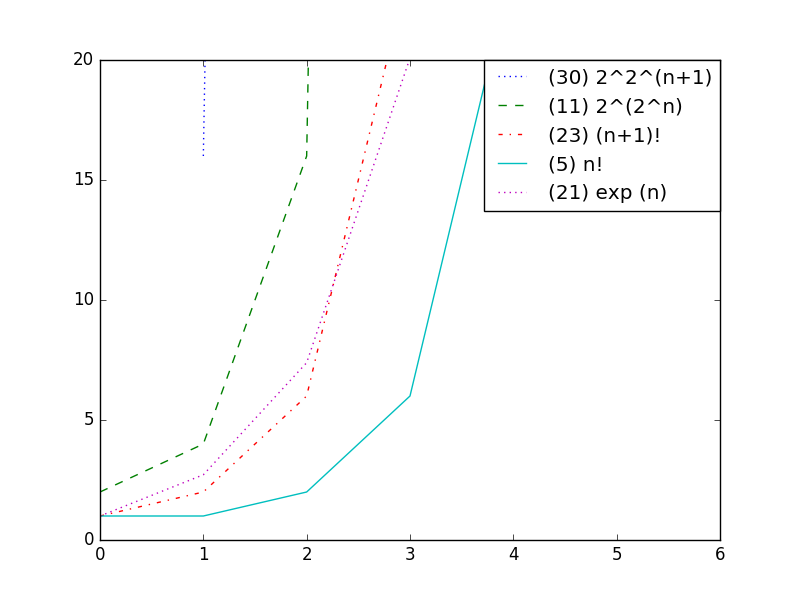
\includegraphics[width=1.1\linewidth, height=4.6cm]{img/figure_6.png} 
%%\caption{Caption1}
\label{fig:subim1}
\end{subfigure}
\begin{subfigure}{0.5\textwidth}
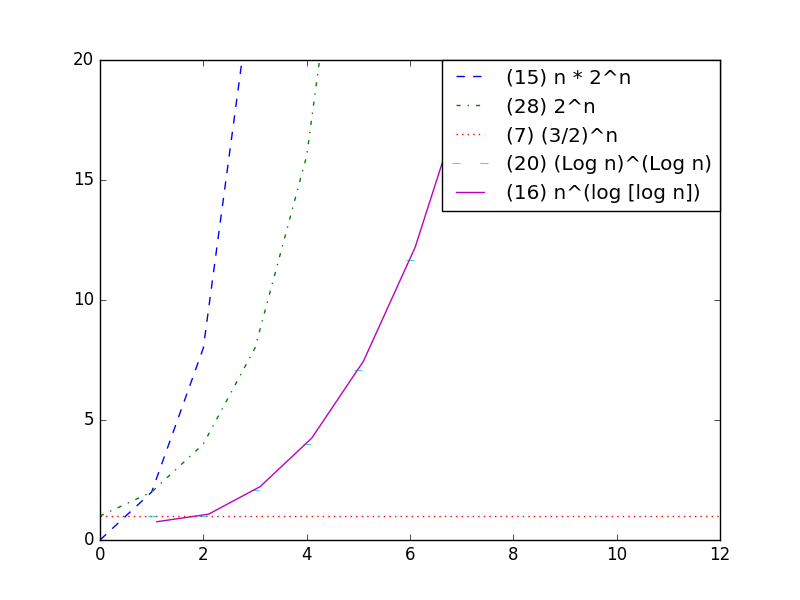
\includegraphics[width=1.1\linewidth, height=4.6cm]{img/figure_5.png}
%%\caption{Caption 2}
\label{fig:subim2}
\end{subfigure}
 
\begin{subfigure}{0.5\textwidth}
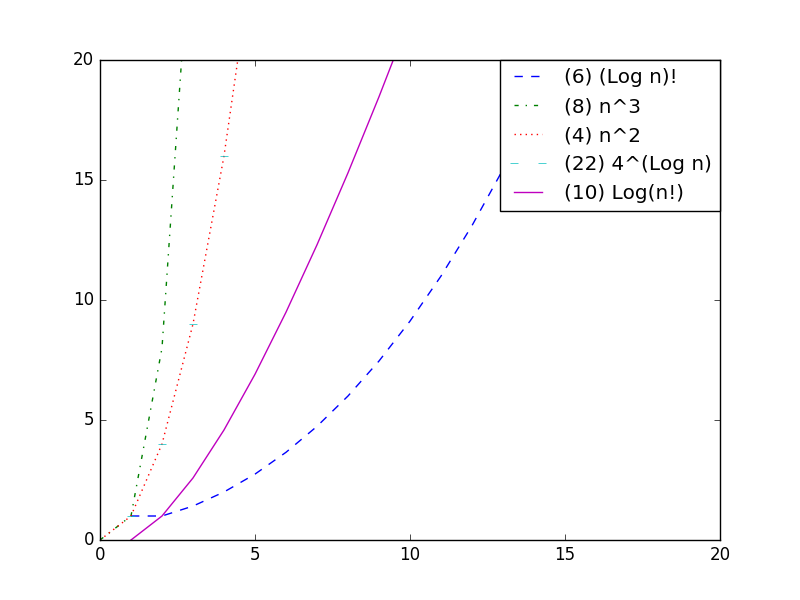
\includegraphics[width=1.1\linewidth, height=4.6cm]{img/figure_4.png} 
%%\caption{Caption1}
\label{fig:subim1}
\end{subfigure}
\begin{subfigure}{0.5\textwidth}
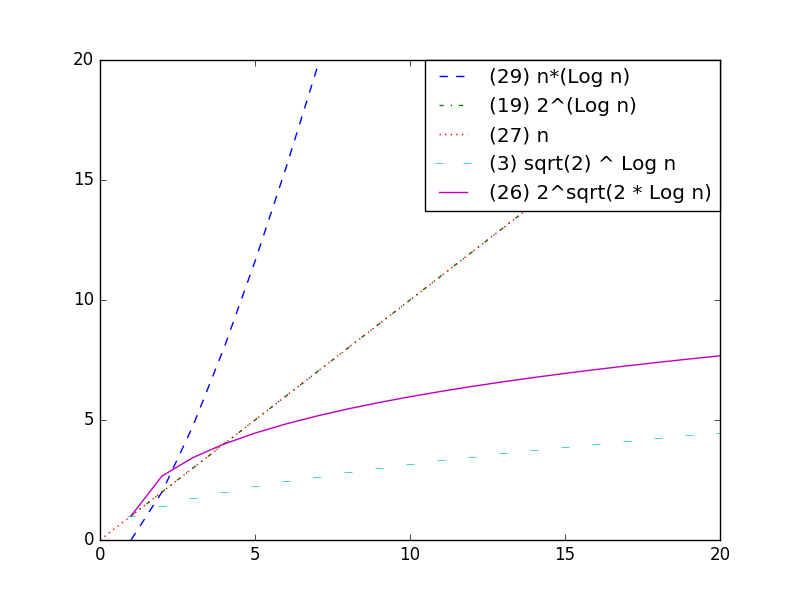
\includegraphics[width=1.1\linewidth, height=4.6cm]{img/figure_3.png}
%%\caption{Caption 2}
\label{fig:subim2}
\end{subfigure}
 
\begin{subfigure}{0.5\textwidth}
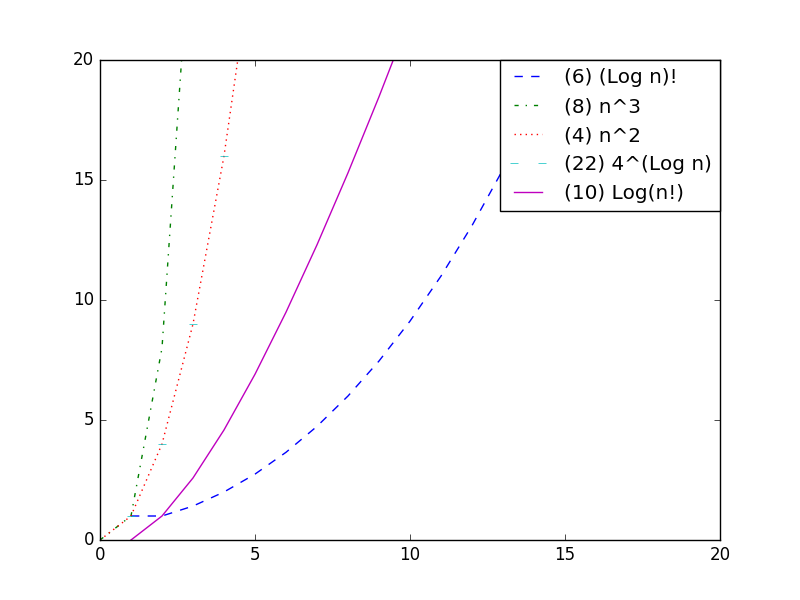
\includegraphics[width=1.1\linewidth, height=4.5cm]{img/figure_4.png} 
%%\caption{Caption1}
\label{fig:subim1}
\end{subfigure}
\begin{subfigure}{0.5\textwidth}
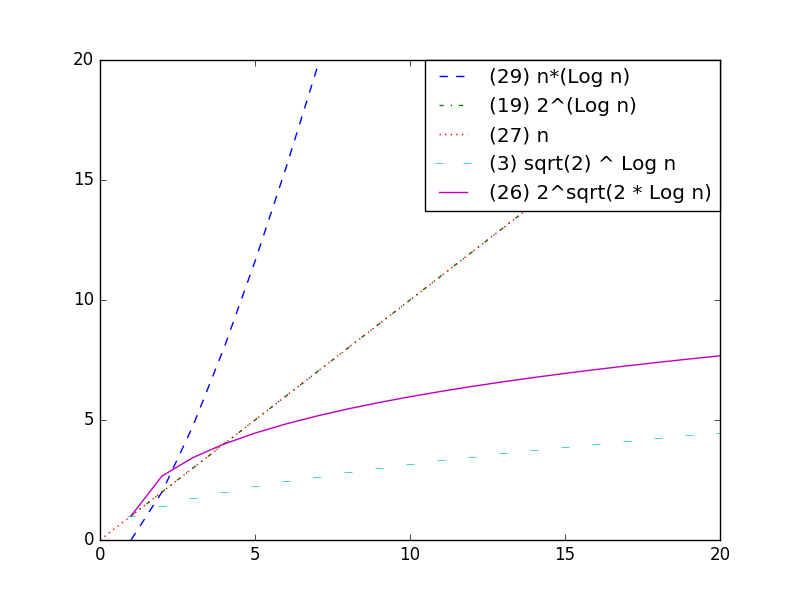
\includegraphics[width=1.1\linewidth, height=4.5cm]{img/figure_3.png}
%%\caption{Caption 2}
\label{fig:subim2}
\end{subfigure}

\label{fig:image2}
\end{figure}

\end{document}

